\documentclass[aspectratio=169]{../latex_main/tntbeamer}  % you can pass all options of the beamer class, e.g., 'handout' or 'aspectratio=43'
\usepackage{dsfont}
\usepackage{bm}
\usepackage[english]{babel}
\usepackage[T1]{fontenc}
%\usepackage[utf8]{inputenc}
\usepackage{graphicx}
\graphicspath{ {./figures/} }
\usepackage{algorithm}
\usepackage[ruled,vlined,algo2e,linesnumbered]{algorithm2e}
\usepackage{hyperref}
\usepackage{booktabs}
\usepackage{mathtools}

\usepackage{amsmath,amssymb}

\DeclareMathOperator*{\argmax}{arg\,max}
\DeclareMathOperator*{\argmin}{arg\,min}

\usepackage{amsbsy}
\newcommand{\vect}[1]{\bm{#1}}
%\newcommand{\vect}[1]{\boldsymbol{#1}}

\usepackage{pgfplots}
\pgfplotsset{compat=1.16}
\usepackage{tikz}
\usetikzlibrary{trees} 
\usetikzlibrary{shapes.geometric}
\usetikzlibrary{positioning,shapes,shadows,arrows,calc,mindmap}
\usetikzlibrary{positioning,fadings,through}
\usetikzlibrary{decorations.pathreplacing}
\usetikzlibrary{intersections}
\pgfdeclarelayer{background}
\pgfdeclarelayer{foreground}
\pgfsetlayers{background,main,foreground}
\tikzstyle{activity}=[rectangle, draw=black, rounded corners, text centered, text width=8em]
\tikzstyle{data}=[rectangle, draw=black, text centered, text width=8em]
\tikzstyle{myarrow}=[->, thick, draw=black]

% Define the layers to draw the diagram
\pgfdeclarelayer{background}
\pgfdeclarelayer{foreground}
\pgfsetlayers{background,main,foreground}

% Requires XeLaTeX or LuaLaTeX
%\usepackage{unicode-math}

\usepackage{fontspec}
%\setsansfont{Arial}
\setsansfont{RotisSansSerifStd}[ 
Path=../latex_main/fonts/,
Extension = .otf,
UprightFont = *-Regular,  % or *-Light
BoldFont = *-ExtraBold,  % or *-Bold
ItalicFont = *-Italic
]
\setmonofont{Cascadia Mono}[
Scale=0.8
]

% scale factor adapted; mathrm font added (Benjamin Spitschan @TNT, 2021-06-01)
%\setmathfont[Scale=1.05]{Libertinus Math}
%\setmathrm[Scale=1.05]{Libertinus Math}

% other available math fonts are (not exhaustive)
% Latin Modern Math
% XITS Math
% Libertinus Math
% Asana Math
% Fira Math
% TeX Gyre Pagella Math
% TeX Gyre Bonum Math
% TeX Gyre Schola Math
% TeX Gyre Termes Math

% Literature References
\newcommand{\lit}[2]{\href{#2}{\footnotesize\color{black!60}[#1]}}

%%% Beamer Customization
%----------------------------------------------------------------------
% (Don't) Show sections in frame header. Options: 'sections', 'sections light', empty
\setbeamertemplate{headline}{empty}

% Add header logo for normal frames
\setheaderimage{
	% 
\includegraphics[height=\logoheight]{figures/TNT_darkv4.pdf}
	
\includegraphics[height=\logoheight]{../latex_main/figures/luh_logo_rgb_0_80_155.pdf}
	% 
\includegraphics[height=\logoheight]{figures/logo_tntluh.pdf}
}

% Header logo for title page
\settitleheaderimage{
	% 
\includegraphics[height=\logoheight]{figures/TNT_darkv4.pdf}
	
\includegraphics[height=\logoheight]{../latex_main/figures/luh_logo_rgb_0_80_155.pdf}
	% 
\includegraphics[height=\logoheight]{figures/logo_tntluh.pdf}
}

% Title page: tntdefault 
\setbeamertemplate{title page}[tntdefault]  % or luhstyle
% Add optional title image here
%\addtitlepageimagedefault{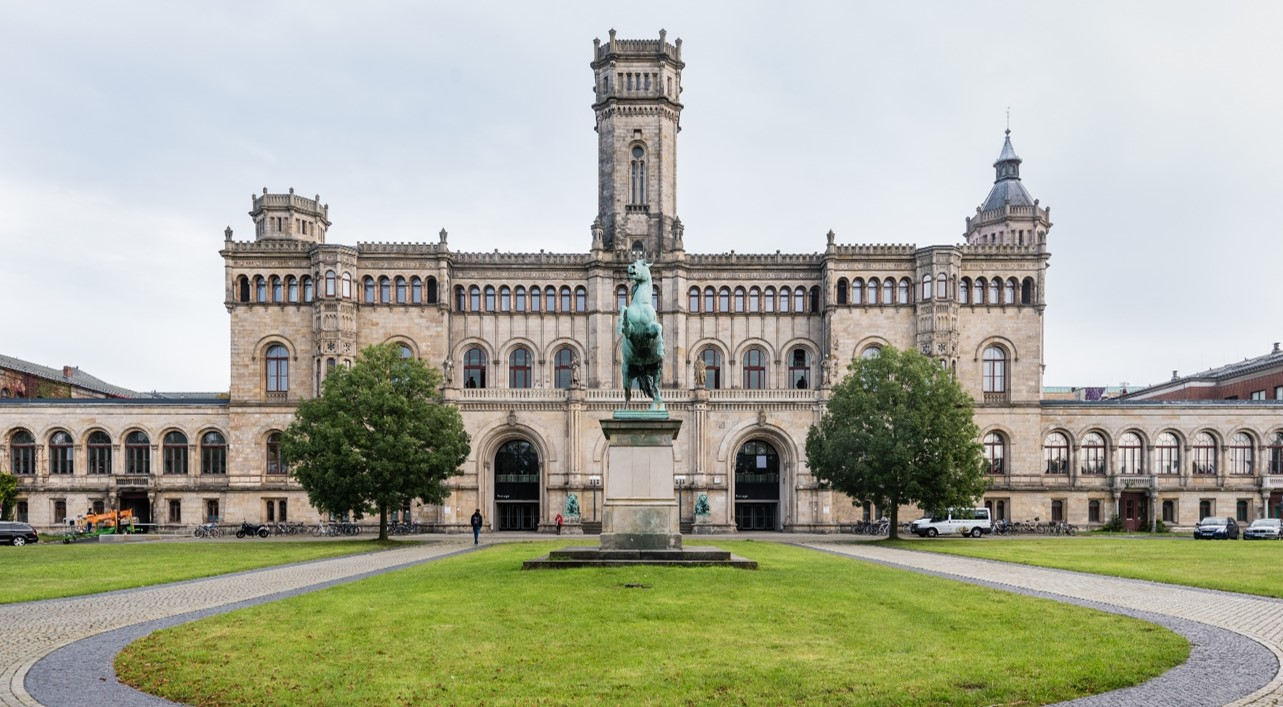
\includegraphics[width=0.65\textwidth]{figures/luh_default_presentation_title_image.jpg}}

% Title page: luhstyle
% \setbeamertemplate{title page}[luhstyle]
% % Add optional title image here
% \addtitlepageimage{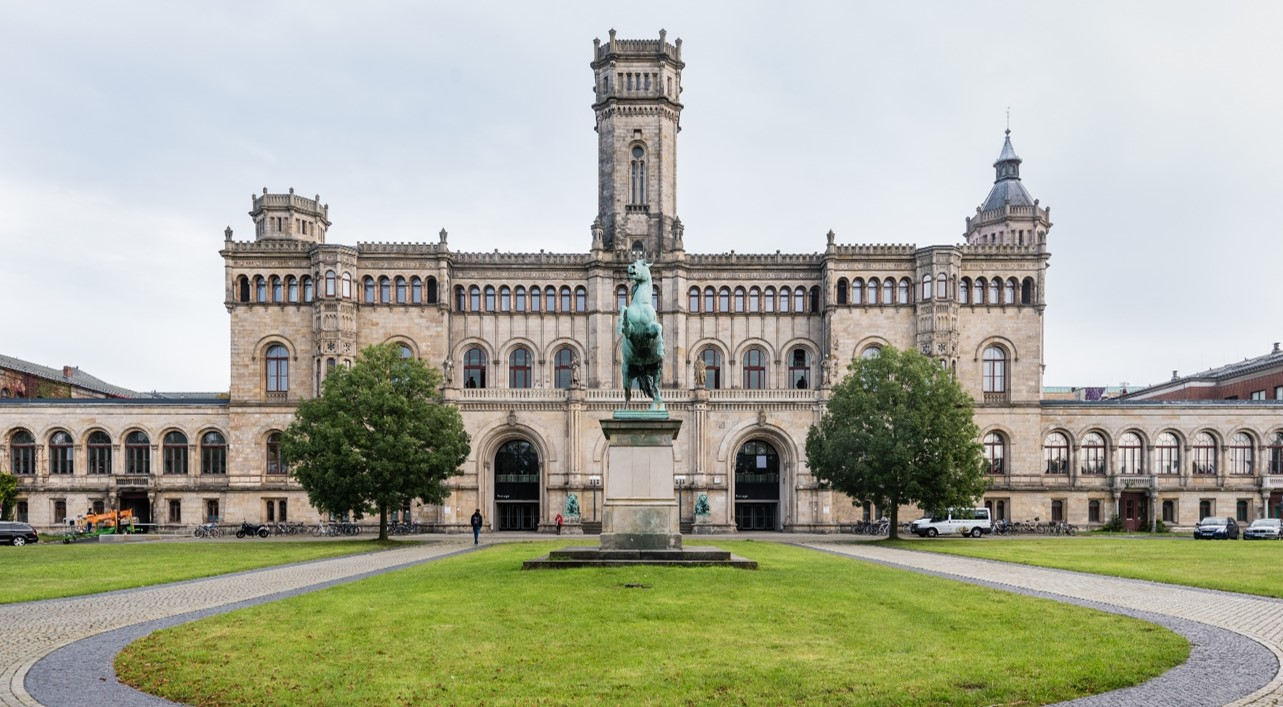
\includegraphics[width=0.75\textwidth]{figures/luh_default_presentation_title_image.jpg}}

\author[Abedjan \& Lindauer]{Ziawasch Abedjan \& Marius Lindauer\\[1em]
	
\includegraphics[height=\logoheight]{../latex_main/figures/luh_logo_rgb_0_80_155.pdf}\qquad
	
\includegraphics[height=\logoheight]{../latex_main/figures/DBIS_Kurzlogo.png}\qquad

\includegraphics[height=\logoheight]{../latex_main/figures/TNT_darkv4}\qquad

\includegraphics[height=\logoheight]{../latex_main/figures/L3S.jpg}	}
\date{Summer Term 2022; \hspace{0.5em} {
\includegraphics[height=1.5em]{../latex_main/figures/Cc-by-nc-sa_icon.svg.png}}; based on \href{https://ds100.org/fa21/}{[DS100]}
}


%%% Custom Packages
%----------------------------------------------------------------------
% Create dummy content
\usepackage{blindtext}

% Adds a frame with the current page layout. Just call \layout inside of a frame.
\usepackage{layout}


%%% Macros
%\renewcommand{\vec}[1]{\mathbf{#1}}
% \usepackage{bm}
%\let\vecb\bm

\title[DL: Training of DNNs]{DS: Deep Learning}
\subtitle{Training of DNNs}

\date{\hspace{0.5em} {
\includegraphics[height=1.5em]{../latex_main/figures/Cc-by-nc-sa_icon.svg.png}}}

\graphicspath{ {./figure/} }
%\institute{}


\begin{document}
	
	\maketitle
	\begin{frame}{Multi-Layer Perceptron Definition}

        Recursive definition of MLPs:

            \[
            \hat{\textbf{y}}^{(l)} = \sigma({\Theta}^{(l)} \hat{\textbf{y}}^{(l-1)} + \textbf{b}^{(l)})
            \]
            
            where:
            \begin{itemize}
                \item \( \hat{\textbf{y}}^{(l)} \) is the output vector from layer \( l \)
                \item \( \Theta^{(l)} \) represents the weight matrix for layer \( l \)
                \item \( \hat{\textbf{y}}^{(l-1)} \) is the output vector from the previous layer \( l-1 \)
                \item \( \textbf{b}^{(l)} \) is the bias vector for layer \( l \)
                \item \( \sigma \) is the activation function (e.g., ReLU)
            \end{itemize}
                
	\end{frame}

        %%%%%%%%%%%%%%%%%%%%%%%%%%%%%%%%%%%%%%%%%%%%%%%%%%%%%%%%%%%%%%
        %%%%%%%%%%%%%%%%%%%%%%%%%%%%%%%%%%%%%%%%%%%%%%%%%%%%%%%%%%%%%%

  	\begin{frame}{Forward Propagation}

        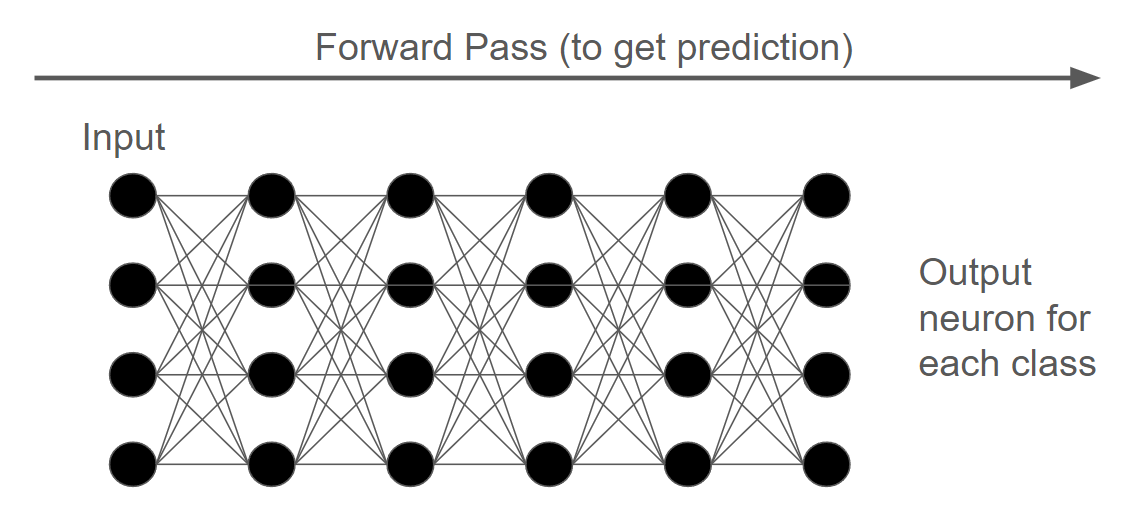
\includegraphics[width=0.8\textwidth]{figures/forward.png}

        \end{frame}

        %%%%%%%%%%%%%%%%%%%%%%%%%%%%%%%%%%%%%%%%%%%%%%%%%%%%%%%%%%%%%%
        %%%%%%%%%%%%%%%%%%%%%%%%%%%%%%%%%%%%%%%%%%%%%%%%%%%%%%%%%%%%%%
  	\begin{frame}{Forward Pass}

        \begin{itemize}
            \item The process of calculating the output from the input layer through to the output layer.
            \item Inputs are processed at each layer using weights, biases, and an activation function.
        \end{itemize}

        
        \begin{block}{Steps of Forward Pass}
        \begin{enumerate}
            \item Start with the input layer \( \hat{\textbf{y}}^{(0)} = \textbf{x} \), where \( \textbf{x} \) is the input vector.
            \item For each layer from 1 to \( L \) (where \( L \) is the output layer):
                \begin{itemize}
                    \item Compute the pre-activation \( \textbf{z}^{(l)} = \Theta^{(l)} \hat{\textbf{y}}^{(l-1)} + \textbf{b}^{(l)} \)
                    \item Apply the activation function \( \hat{\textbf{y}}^{(l)} = \sigma(\textbf{z}^{(l)}) \)
                \end{itemize}
            \item The final output \( \hat{\textbf{y}}^{(L)} \) is the prediction of the network.
        \end{enumerate}
        \end{block}
                
	  \end{frame}

        %%%%%%%%%%%%%%%%%%%%%%%%%%%%%%%%%%%%%%%%%%%%%%%%%%%%%%%%%%%%%%
        %%%%%%%%%%%%%%%%%%%%%%%%%%%%%%%%%%%%%%%%%%%%%%%%%%%%%%%%%%%%%%
  	\begin{frame}{Backpropagation: I}

        \vspace{-2em}
        \begin{itemize}
            \item Backpropagation is used to calculate the gradient of the loss function of a DNN wrt its weights.
            \item Key algorithm used in training DNN, allowing for efficient computation of gradients.
        \end{itemize}
        
        \begin{block}{Error Term Calculation}
        For each output neuron \( k \), the error \( \delta_k \) is computed as:
        \[
        \delta_k = \frac{\partial \mathcal{L}}{\partial \hat{y}_k^{(L)}} \sigma'(z_k^{(L)})
        \]
        where:
        \begin{itemize}
            \item \( \mathcal{L} \) is the loss function.
            \item \( \hat{y}_k^{(L)} \) is the activation of the \( k \)-th neuron in the output layer.
            \item \( \sigma' \) is the derivative of the activation function.
            \item \( z_k^{(L)} \) is the input to the activation function in the output layer.
        \end{itemize}
        \end{block}

        \end{frame}
        %%%%%%%%%%%%%%%%%%%%%%%%%%%%%%%%%%%%%%%%%%%%%%%%%%%%%%%%%%%%%%
        %%%%%%%%%%%%%%%%%%%%%%%%%%%%%%%%%%%%%%%%%%%%%%%%%%%%%%%%%%%%%%
  	\begin{frame}{Backpropagation: II}

        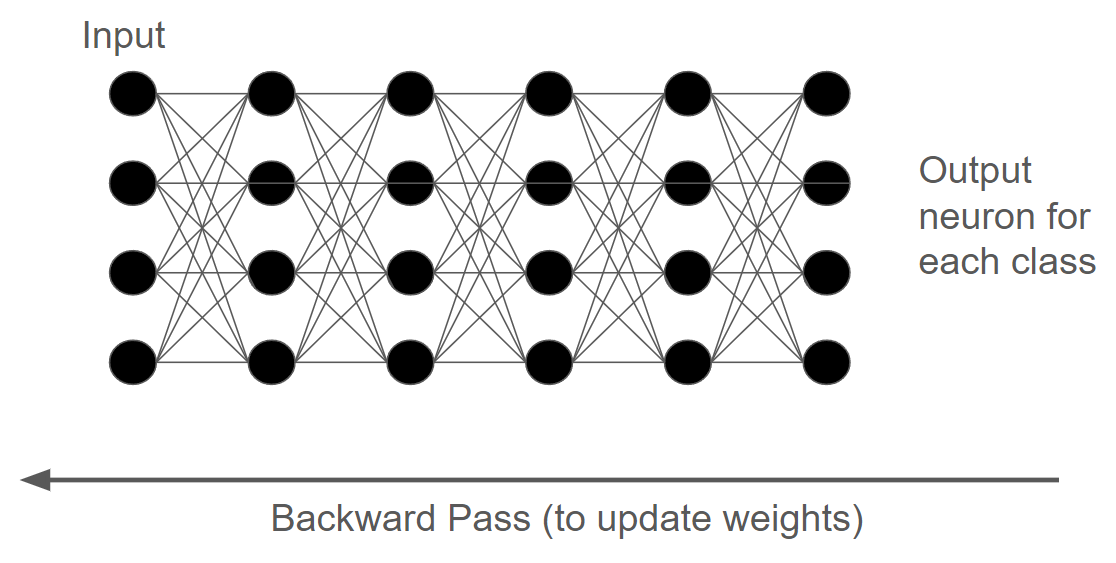
\includegraphics[width=0.8\textwidth]{figures/backward.png}

        \end{frame}
        %%%%%%%%%%%%%%%%%%%%%%%%%%%%%%%%%%%%%%%%%%%%%%%%%%%%%%%%%%%%%%
        %%%%%%%%%%%%%%%%%%%%%%%%%%%%%%%%%%%%%%%%%%%%%%%%%%%%%%%%%%%%%%
        \begin{frame}{Backpropagation: III}

        \vspace{-2em}
        \begin{block}{Gradient Computation for Weights}
        The gradient of the loss with respect to the weights is given by:
        \[
        \frac{\partial \mathcal{L}}{\partial \Theta_{ij}^{(l)}} = \hat{y}_j^{(l-1)} \delta_i^{(l)}
        \]
        where:
        \begin{itemize}
            \item \( \Theta_{ij}^{(l)} \) are the weights connecting Neuron \( j \) in Layer \( l-1 \) to Neuron \( i \) in Layer \( l \).
            \item \( \delta_i^{(l)} \) is the error term for Neuron \( i \) in Layer \( l \).
        \end{itemize}
        \end{block}

        Important to note: Backpropagation makes use of the chain rule of calculus (see optional slide at the end)
        
        \end{frame}
        %%%%%%%%%%%%%%%%%%%%%%%%%%%%%%%%%%%%%%%%%%%%%%%%%%%%%%%%%%%%%%
        %%%%%%%%%%%%%%%%%%%%%%%%%%%%%%%%%%%%%%%%%%%%%%%%%%%%%%%%%%%%%%
        \begin{frame}{Update Rule}

        \begin{block}{Update Rule}
            Weights are updated using the rule:
            \[
            \Theta_{ij}^{(l)} \leftarrow \Theta_{ij}^{(l)} - \eta \frac{\partial \mathcal{L}}{\partial \Theta_{ij}^{(l)}}
            \]
            where \( \eta \) is the learning rate.
         \end{block}
            
        \end{frame}

        %%%%%%%%%%%%%%%%%%%%%%%%%%%%%%%%%%%%%%%%%%%%%%%%%%%%%%%%%%%%%%
        %%%%%%%%%%%%%%%%%%%%%%%%%%%%%%%%%%%%%%%%%%%%%%%%%%%%%%%%%%%%%%
        \begin{frame}{The Chain Rule in Backpropagation (Optional Slide)}

        \vspace{-2em}
        \begin{itemize}
            \item The chain rule of calculus is essential for how gradients are computed in backpropagation.
            \item Backpropagation uses the chain rule to find the derivatives of the loss function with respect to each weight in the network by propagating errors back from the output towards the input layer.
        \end{itemize}
        
        \begin{itemize}
            \item To update the weight \( w_{ij}^{(l)} \), we need to compute:\\
            $
            \frac{\partial \mathcal{L}}{\partial \Theta_{ij}^{(l)}} = \frac{\partial \mathcal{L}}{\partial \hat{y}_i^{(l)}} \cdot \frac{\partial \hat{y}_i^{(l)}}{\partial z_i^{(l)}} \cdot \frac{\partial z_i^{(l)}}{\partial \Theta_{ij}^{(l)}}
            $
            \item Where:
            \begin{itemize}
                \item \( \frac{\partial \mathcal{L}}{\partial \hat{y}_i^{(l)}} \) is the derivative of the loss function with respect to the activation of neuron \( i \) in layer \( l \).
                \item \( \frac{\partial \hat{y}_i^{(l)}}{\partial z_i^{(l)}} \) is the derivative of the activation function at \( z_i^{(l)} \).
                \item \( \frac{\partial z_i^{(l)}}{\partial w_{ij}^{(l)}} \) is the input from neuron \( j \) in the previous layer \( l-1 \).
            \end{itemize}
            \item This decomposition allows us to update all the weights $\Theta$ in a single backward pass
        \end{itemize}

        \end{frame}

 	
\end{document}